\section{系统实现与交互}\label{sec:implementation}
\ChapterOwner{B}{C、D}
\subsection{工程组织与实现环境}
\Writing{B}{主要目录、职责、锁定版本与构建方式，不抄全部依赖。}
\subsection{真实用户操作实例}
\Writing{B}{沿提问、查看来源、组合检索、回原会话、作答、查看成长依据，选 6--8 张真截图。每图写日期、操作/输入/输出、相关表、demo/live/预置。以下仅为现有运行材料接入示例，应按最终版本更新。}
\begin{figure}[htbp]\centering
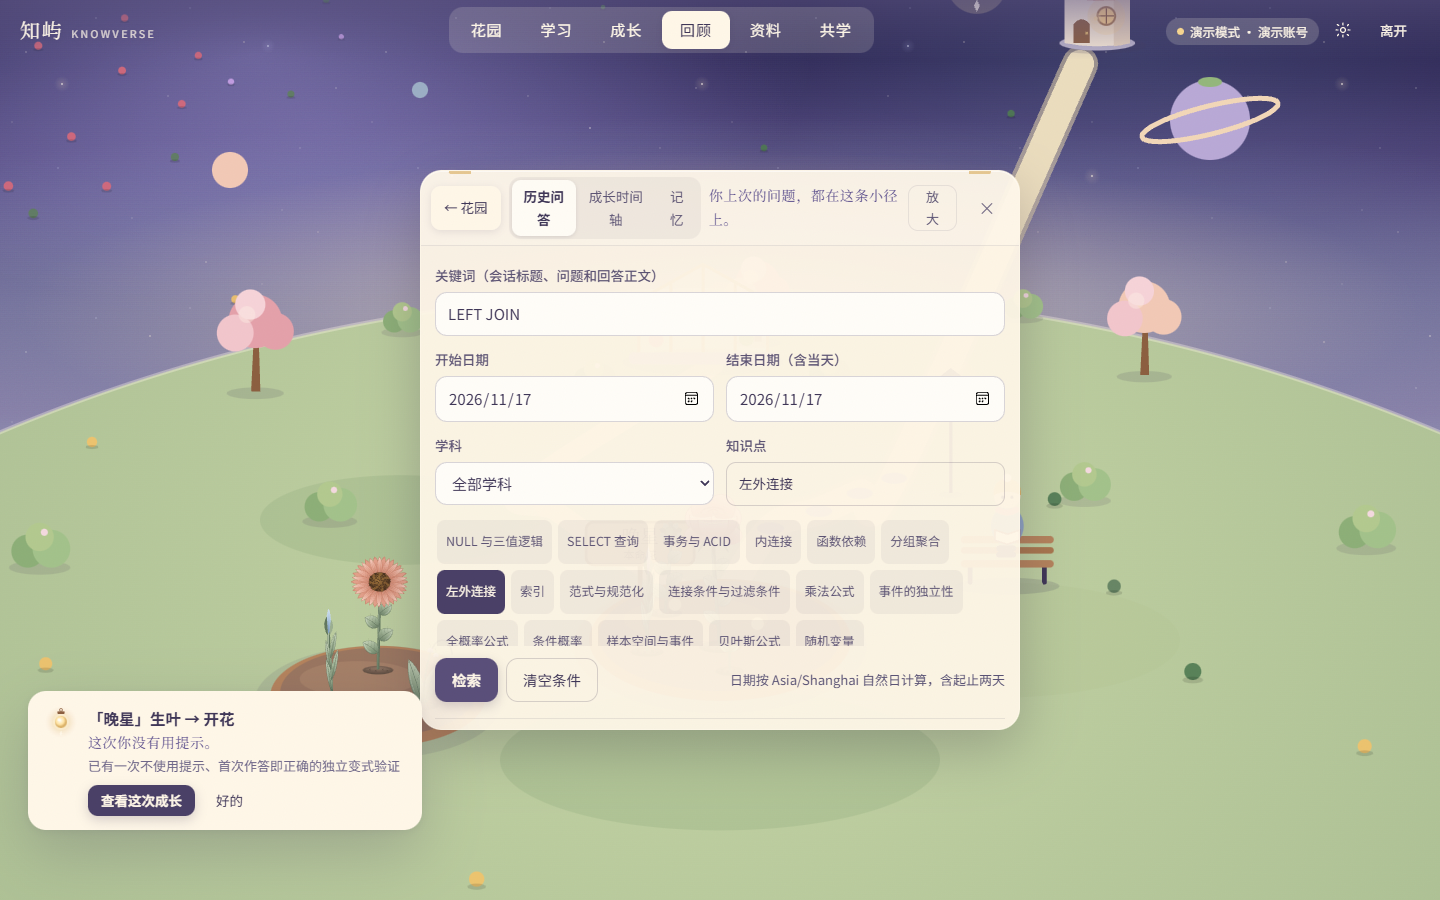
\includegraphics[width=.93\linewidth]{../../screenshots/acceptance-2026-11-17/09-history-combined.png}
\caption{2026-11-17 真实浏览器验收截图：组合历史检索；demo 模式、静态绘本降级}\label{fig:history-shot}
\end{figure}
\FloatBarrier
\subsection{数据库状态到界面的映射}
\Writing{B，A 核对}{概念与植物、学习状态与阶段、证据与成长说明怎样映射。数据事实驱动界面，不能倒写为动画驱动结算。}
\subsection{异常处理与反馈}
\Writing{B}{等待、模型失败、资料不足、引用不通过、无结果、重复提交、沙箱不可用等状态和实际反馈。}
\subsection{响应式、可访问性与降级}
\Writing{B}{移动、键盘、低动效、无 WebGL；班级为 2D SVG，主花园与降级另述。软件渲染截图不推导真机帧率。}
\subsection{实现难点与取舍}
\Writing{B}{选 2--3 个真实问题讲原因、修改、回归与剩余限制。HTML 动画只是流程示意，不替代真实截图或性能记录。}
\Evidence{docs/screenshots/acceptance-2026-11-17/; docs/screenshots/ui/; docs/visual-redesign.md}
